\chapter{Visão Geral}
    \section{Perspectiva do Produto}
        \par O produto visa atender qualquer casa, direcionado a clientes dispostos a alterar sua casa em prol da economia e sustentabilidade , e também visa atender ao maior número de pessoas. Com isso teria uma  possível melhora na produção e economia energética da cidade, tendo uma maior independência energética gerando possivelmente até lucro ao cliente e a cidade.

        \subsection{Conceitos Relevantes}
            \subsubsection{Smart Grid}
                \par O conceito de \textit{Smart Grid} que foi descrito por Amin e Wollenberg (2005) é definido como “uma infraestrutura de rede elétrica em larga escala caracterizada por segurança, agilidade, resiliência/robustez que enfrenta novas ameaças e condições não previstas”[Amin e Wollenberg (2005, p.1)]. É um novo sistema de distribuição e transmissão de energia elétrica que funciona com o uso de recursos tecnológicos avançados, baseados em equipamentos digitais integrados. A maior eficiência e a facilidade de gestão energética oferecida pela \textit{Smart Grid} fazem com que esse sistema seja capaz de atender a diversos tipos de demandas e necessidades exigidas em grandes centros urbanos e industriais. \cite{aminwollenberg2005}
                \par Em resumo, e durante a realização desse projeto, o objetivo das smart grids é otimizar a produção e o consumo de energia na residência onde for aplicada.
                \par Um dos principais componentes desse complexo de redes é o medidor eletrônico inteligente, que substitui o tradicional medidor analógico. Esse equipamento oferece uma série de novas funcionalidades, como o envio de dados em tempo real, medição remota, sistema de alarme de sobrecarga da rede, além dos ajustes automáticos de economia de energia. Tudo isso permite um acompanhamento mais minucioso do consumo, tanto por parte das empresas de energia quanto pela população em geral. \cite{ecycle}
                \par Do ponto de vista ambiental, a \textit{Smart Grid} oferece uma série de benefícios ao ser capaz de reconhecer instantaneamente uma queda no fornecimento da rede e realizar, de modo automático, todas as medidas necessárias para o restabelecimento da distribuição. Essas ações, juntos com um controle mais rígido sobre fraudes e desvios, diminuem bastante o desperdício de energia.  Além disso, as redes inteligentes se integram facilmente com fontes renováveis de energia, tanto para consumidores de baixa tensão (setor residencial) quanto para os de alta tensão (comércios e indústrias). \cite{siemens}
            \subsubsection{Internet das Coisas}
                \par O termo Internet das Coisas (IoT) foi criado e introduzido à humanidade por um dos pioneiros tecnológicos atuais chamado Kevin Ashton, que, por meio de sensores “onipresentes” conseguiu conectar o mundo físico à Internet. Utilizando mecanismos eletrônicos como Raspberry ou Arduinos, que permite a conexão com a Internet e serve como um centro de controle, é possível construir objetos como geladeira, fogão, sistema de iluminação, portão, porta, cafeteira, sistema de irrigação, jardinagem, etc, para serem “coisas” conectadas à internet, e isso abre portas para uma gama de possibilidades onde o limite é a criatividade e, é claro, o custo. A principal ideia de conseguir conectar objetos físicos com a Internet é permitir que tais objetos ou um conjunto deles sejam manipulados por meio de uso remoto, ou seja, sem que haja a necessidade de estar no mesmo local do objeto para poder utilizá-lo ou controlá-lo.
                \par O avanço de outros tipos de tecnologias, como algoritmos de inteligência artificial trazem um enorme avanço na IoT, visto que pode-se construir não somente objetos conectados à internet e sim os chamados smart objects ou objetos inteligentes, que visam realizar atividades por uso de machine learning e aprendizado de padrões. Um exemplo não muito inteligente seria uma cafeteira que, por alguns dias identifica um padrão de comportamento de seu usuário e identifica os horários específicos de cada dia da semana que o mesmo costuma tomar seu café. Com isso, a máquina consegue “aprender” sobre o seu “dono” e, sem que o mesmo tenha que solicitar o café, a máquina já deixará pronto nas horas de costume.
                \par Um outro ponto interessante é o uso de sensores juntamente com a internet das coisas, visto que é possível uma via de mão dupla: não só o usuário envia comandos para serem executados pelas “coisas”, mas elas podem detectar alguns sinais por meios de sensores e dizer ao usuário que necessitam fazer algo. Por exemplo: um jardim que possui diversas plantas e um sistema de irrigação. Pode existir um sensor que observa a umidade do solo para saber se as plantas precisam ou não de irrigação. Com isso, é possível o sistema de controle de irrigação notifique o usuário que o solo está em um nível que necessite de água, permitindo que o usuário responda com uma ordem ou comando, e, assim, o sistema realize a tarefa de irrigar o jardim.

    \section{Estruturas e Materiais}
        \subsection{Local}
            \par A residência estudada se localiza na Região do Riacho Fundo I, com um tamanho de 160 metros quadrados, atendendo todas as especificações do projeto.
            \par Seus cômodos são: sala, cozinha, quartos, banheiros, escritório, garagem, área de serviço e varanda.

        \subsection{Construção Sustentável}
            \par A construção sustentável é uma forma de se construir casa e edifícios, harmonizando-os com o meio ambiente.Esse tipo de construção busca amenizar os impactos à natureza, reduzindo o máximo possível de resíduos e utilizando com eficiência os materiais e bens naturais, como energia e água. \cite{ecycle}
	        \par Com o objetivo de tornar a casa sustentável, serão utilizados materiais que potencializam a eficiência térmica e energética da casa, além da utilização materiais recicláveis e de menor impacto ambiental, como madeiras reflorestadas e tijolo de adobe, por exemplo.
        \subsection{Materiais}
            \par Para as paredes, serão utilizados:
                \begin{itemize}
                    \item Reboco, tipo de argamassa para deixar as paredes uniformes e aptas a receber a tinta;
                    \item Tinta Pva látex, a base de acetato de polivinila, uma tinta solúvel em agua de fácil utilização a facilmente encontrada no mercado;
                    \item Azulejo, material cerâmico utilizado para revestir pisos e paredes, impermeável e facilmente limpável.
                \end{itemize}
            \par Para os pisos, serão utilizados:
                \begin{itemize}
                    \item Azulejo, material cerâmico utilizado para revestir pisos e paredes, impermeável e facilmente limpável;
                    \item Calçada de concreto magro, calçamento feito de concreto com pouco cimento. Sem funções estruturais, utilizado apenas como contra piso.
                \end{itemize}
            \par Para o teto, serão utilizados:
                \begin{itemize}
                    \item Laje com reboco
                    \item Tinta Pva látex, a base de acetato de polivinila, uma tinta solúvel em agua de fácil utilização a facilmente encontrada no mercado.
                \end{itemize}
            \par Para a cobertura, serão utilizadas:
                \begin{itemize}
                    \item Telhas de cerâmica, feita de argila queimada, facilmente encontrado no mercado e proporciona bom isolamento térmico e acústico com um bom custo benefício.
                \end{itemize}

	   \subsection{Planta Baixa da Residência Modelo}
	   % Planta da Casa
        \graphicspath{ {figuras/} }
        \begin{figure}[h]
            \centering
            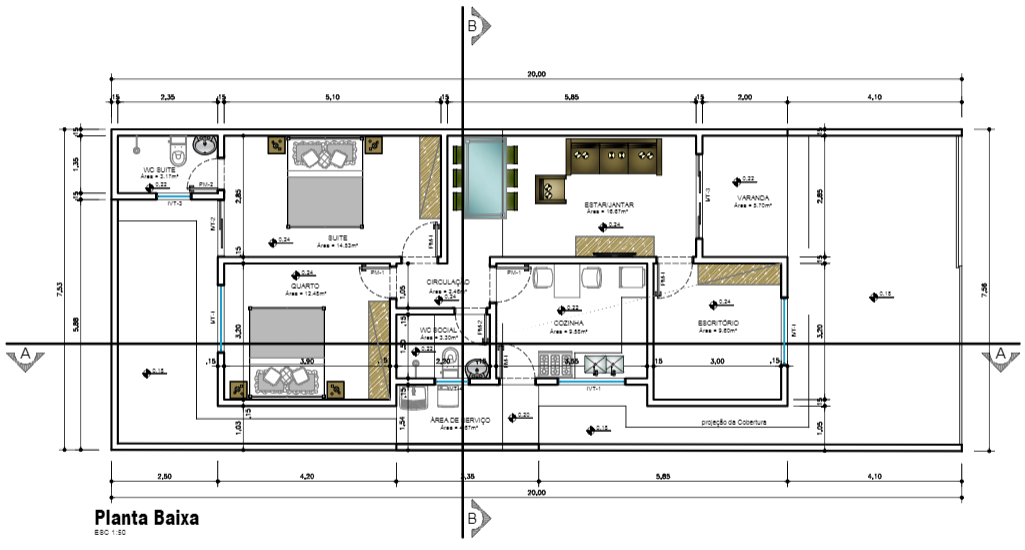
\includegraphics[scale=0.5]{planta}
            \caption{Planta da Casa}
            \label{fig:planta}
        \end{figure}

	   \section{Sistema Energético}
	       \subsection{Fonte de Energia}
	           \begin{itemize}
        	       \item Qual fonte de energia vai ser utilizada?
            	       \begin{itemize}
            	            \item A principal fonte de energia utilizada na casa vai ser proveniente de placas solares.
            	       \end{itemize}
        	       \item Por quê?
        	            \begin{itemize}
        	                \item Incentivos governamentais
        	                    \par O governo tem incentivado muito o uso dessas fontes de energia, seja por meio de subsídios à indústria que produz os equipamentos para sua geração, seja por meio da regulamentação de seu uso (Residencial).
        	                \item Sustentabilidade ambiental
        	                    \par Essa é a principal vantagem da energia solar fotovoltaica como fonte energética. Primeiramente, ela reduz a utilização de outras fontes de energia, como a hidrelétrica (Provinda das concessionárias) e o gás. \cite{solarvolt}
                                \par É importante notar que algumas dessas fontes de energia substituídas não são renováveis, o que significa que haverá sua escassez no futuro.
                                \par A energia solar é abundante e pode ser encontrada com facilidade e regularidade em boa parte do país. Além disso, seus impactos sobre o meio ambiente são muito baixos, pois não há emissão de resíduos poluentes, nem apresenta riscos à saúde das pessoas da casa.
                            \item Economia de recursos
                                \par A economia de recursos está relacionada não apenas aos recursos ambientais (gás natural, petróleo, eletricidade), mas também à diminuição dos custos com despesa elétrica.
                                \par O investimento inicial na compra de equipamentos para captura de energia solar e eólica é rapidamente coberto por meio da economia gerada no futuro, além de que os custos de manutenção são bastante baixos. Além disso, no caso da energia solar, a vida útil dos painéis é de 40 anos, o que representa um investimento rentável e duradouro.
                            \item Facilidade de instalação
                                \par A instalação de sistemas de captura de energia solar fotovoltaica é fácil e rápida, por isso é chamada de plug-and-play (conectar e utilizar, em inglês).
                                \par Sua instalação interfere muito pouco no sistema elétrico já existente no imóvel, além de servir de acordo com as necessidades da família. Como o sistema é modular, pode-se instalar um número X de painéis e, caso necessário, mais painéis poderão ser instalados no futuro sem grandes dificuldades.
        	            \end{itemize}
        	       \item Como vai ser utilizada essa energia?
	                    \begin{itemize}
	                        \item O sistema adotado para utilização da energia produzida foi o Sistema conectado a rede ou on-grid, em que depois de produzida a energia nas placas solares, a corrente vai passar por um inversor para converter a corrente contínua em corrente alternada, e em seguida essa energia será direcionada para o sistema elétrico da casa e ao medidor da rede. Quando a geração solar fotovoltaica for superior a demanda, o sistema injeta essa energia em excesso na rede, gerando um saldo líquido para ser utilizado quando a geração fotovoltaica for inferior a demanda e no período noturno. Assim o saldo líquido gerado vai compensar esses déficits.
	                    \end{itemize}
        	        \end{itemize}
        	 \subsection{Armazenamento de Energia}
        	    \par Mesmo a principal fonte de energia sendo solar, é necessário um sistema que armazene parte dessa energia para uma possível queda de energia. Levantando essa possibilidade, acoplado ao sistema elétrico da casa, conterá uma bateria que vai fornecer energia para um sistema crítico, ou seja, mesmo após a queda de energia, alguns equipamentos e a parte de automação continuará funcionando.
                \par Será utilizado a energia produzida nas próprias placas fotovoltaicas para recarregar a bateria.

            \subsection{Captação da Água da Chuva}
                \par Serão feitas através  de calhas instaladas ao redor da casa e direcionadas para um tanque, logo depois serão repassadas para os sistemas responsáveis pela parte de reutilização. Esses tanques serão compostos de sensores que estarão programados para mandar avisos ao cliente através do aplicativo, contendo informações de cunho relevante, por exemplo: Após atingir uma determinada altura os sensores ativam o sistema de irrigação de plantas. Entre outros comandos definidos para o projeto. Assim, além de uma casa tecnológica, será possível obter um projeto sustentável, visando melhor qualidade e uma diminuição nos gastos mensais do cliente. \cite{ecycle}

            \subsection{Reutilização da Água}
                \par A casa terá um sistema de reutilização da água proveniente do chuveiro, pia do banheiro e máquina de lavar para ser utilizada em outras atividades, como regar o jardim, lavagem de pisos e descarga do vaso sanitário.
 	            \par O projeto conta com vasos sanitários econômicos, com isso o uso de água será limitado (cerca de 6 litros por descarga),  assim, será possível reduzir seu consumo quase pela metade, já que uma descarga antiga utiliza 10 litros de água e no uso de válvulas utiliza-se quase o dobro. Alternativa já presente nos mercados.  A água utilizada nos banhos, será desviada do ralo para um cano com filtros,  ligado diretamente com o reservatório acoplado ao vaso sanitário. \cite{sociedadedosol}
 	            \par Já no caso da água usada nas outras atividades citadas, a água também será desviada para um reservatório com filtros e tratamentos que vai estar ligada também em no sistema de irrigação do jardim, que será ativado em uma certa hora do dia ou em uma certa quantidade x armazenada no tanque. O uso será usada também na limpeza dos pisos da varanda e da garagem.

 	      \section{Sistema de Automação}
 	        \subsection{Integração com Smart Grid e Internet das Coisas}
 	            \par Todos os equipamentos da casa estarão interconectados, e com as informações de eficiência disponibilizadas pelo aplicativo será possível definir parâmetros de  consumo e assim maximizar a eficácia de todo o sistema.

 	        \subsection{Controle Energético}
	            \par O controle energético será feito por meio de um medidor inteligente interligado  no aplicativo que será capaz de controlar quanto de energia está sendo consumida e quanto está sendo injetada na rede, quais os equipamentos que estão consumindo mais energia e uma possível estimativa de fatura caso não seja possível zerar a conta por meio da produção de energia pelas células fotovoltaicas. \cite{solarvolt}

	       \subsection{Controle Energético}
	            \par Será utilizado um aplicativo que receberá todos os dados da parte de automatização e, além de disponibilizar dados de temperatura, umidade entre outros, possibilitará o cliente fazer as alterações que ele desejar, como ligar ou desligar luzes, abrir a cortina, definir a temperatura desejada do cômodo, entre outras possibilidades. além de alertas de segurança, como possibilidade de incêndio e invasão da casa.

	       \subsection{Segurança}
	            \par Na parte de segurança, caso haja um sistema previamente instalado, faremos a comunicação com o aparelho e nosso aplicativo integrando os dois. Ou também há a alternativa de uma parceria com empresas de sistema de segurança.

	       \subsection{Sensores}
	            \par Os principais sensores presentes na casa são so sensores de presença, luminosidade, gás, fumaça, temperatura e umidade. Cada um terá respostas para dadas situações.
	            \par Os sensores foram distribuídos por tipo de cômodo visando que cada cômodo tem sua peculiaridades:
	            \begin{itemize}
	                \item Sala e Quartos: presença, fumaça, umidade, temperatura e luminosidade
                    \item Cozinha: gás, presença, fumaça, umidade, temperatura e luminosidade
                    \item Banheiro: presença, fumaça e luminosidade
                    \item Área de Serviço: fumaça e presença
	            \end{itemize}
	            \subsubsubsection{Sensor de Gás}
	                \par Vai monitorar a presença de gás na cozinha avisando ao usuário quando estiver vazando e aciona o exaustor da cozinha para dissipar o gás presente no ambiente.
	            \subsubsubsection{Sensor de Temperatura/Umidade}
	                \par Vai monitorar a temperatura ou a umidade do ambiente no qual está instalado, ao receber o comando para o ambiente ficar em determinada temperatura vai acionar o ar condicionado.
	            \subsubsubsection{Sensor de Presença}
	                \par Verifica a presença de pessoas em cômodos, funciona conforme movimento se as pessoas no local ficarem determinada quantidade de tempo sem apresentar movimento o mesmo vai agir nos atuadores desativando a iluminação local, contudo ele não irá retomar as luzes caso a pessoa se mova, também fará parte do sistema de segurança quando acionado nesta função, o alarme será ativado quando o sensor detectar a presença de alguém em área predefinidas.
	            \subsubsubsection{Sensor de Fumaça}
	                \par Vai identificar a fumaça,acionando o sistema contra incêndio da casa, acionando um alarme de incêndio, liberando água para o quarto que tenha o seu sensor acionado e por meio de um sprinkler tentar apagar ou reduzir o foco de incêndio, até a chegada da brigada de incêndio ou bombeiros que foi chamado ao mesmo tempo que foi acionado o alarme.

	   \section{Aplicativo}
 	        \subsection{Resumo}
 	            \par O aplicativo será capaz de mostrar o consumo energético, controlar a temperatura dos cômodos desejados e também controlará objetos eletrônicos, como televisão e geladeira.
 	        \subsection{Ícone}
     	        % ícone
                \graphicspath{ {figuras/} }
                \begin{figure}[h]
                    \centering
                    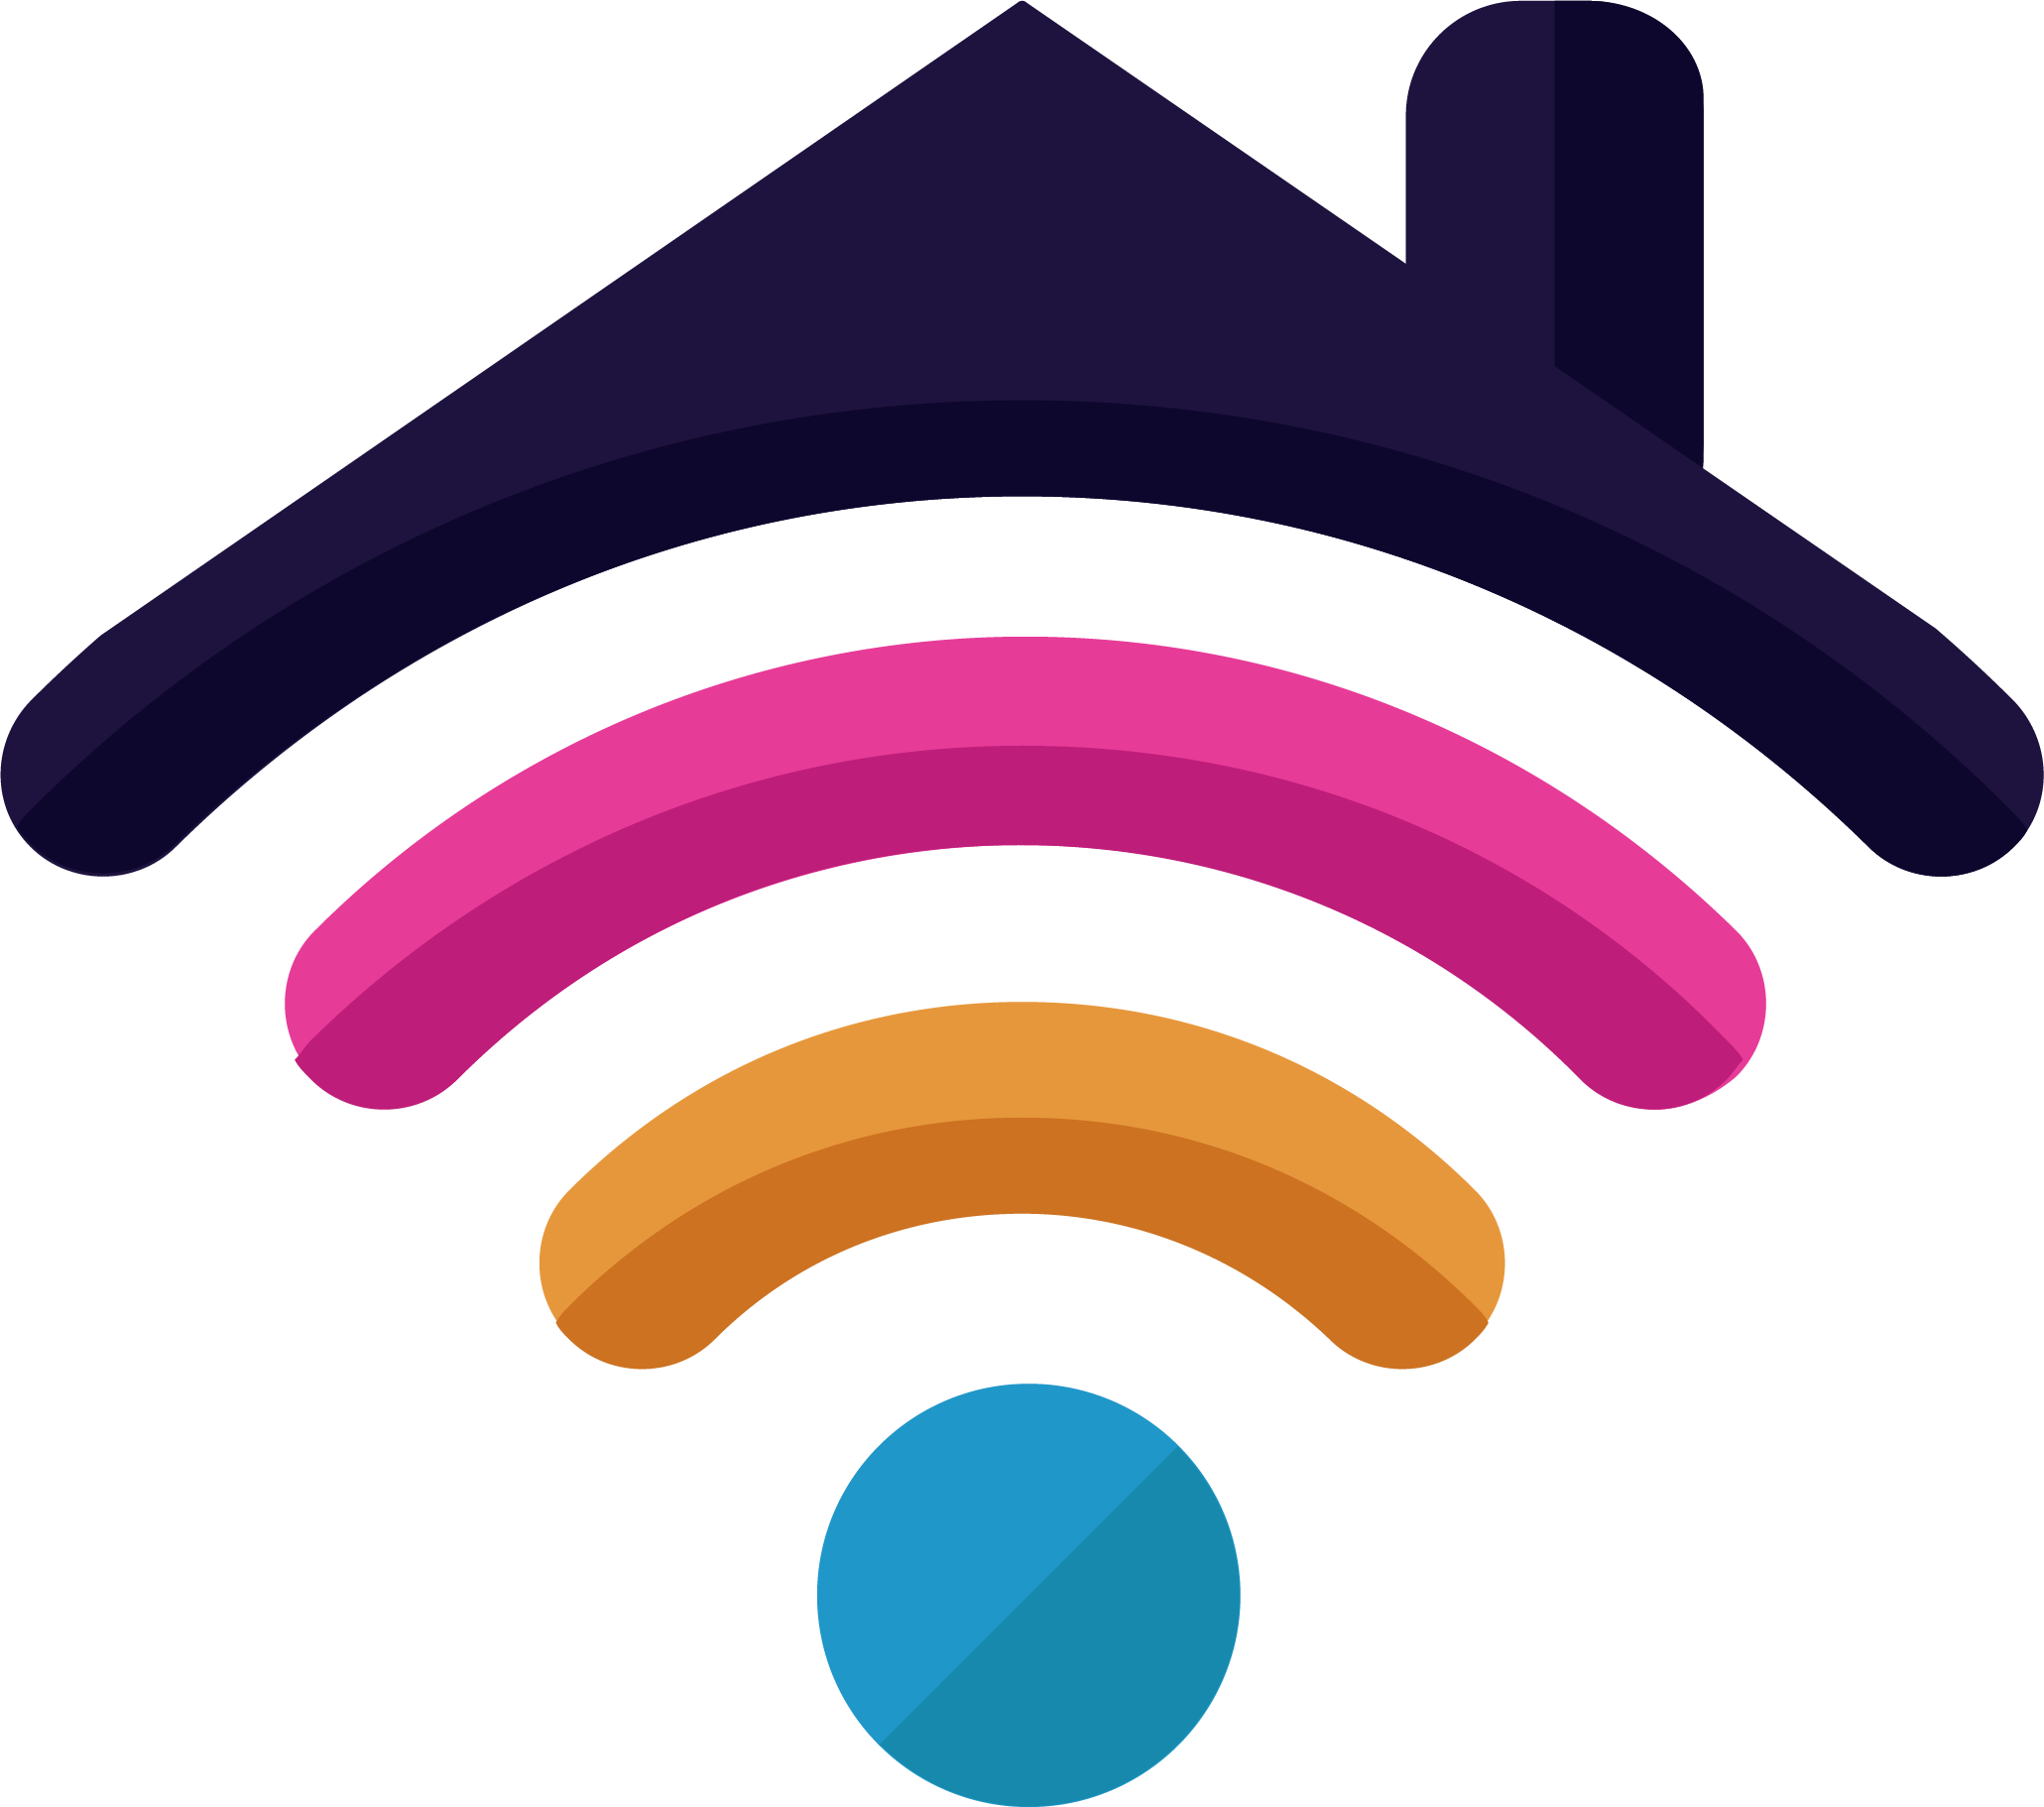
\includegraphics[scale=0.4]{icon}
                    \caption{Ícone do Aplicativo}
                    \label{fig:icon}
                \end{figure}
 	        \subsection{Protótipo}
 	            \par Foi criado um protótipo simples para simular o fluxo de telas da aplicação e a sua interface. Além disso, contém a paleta de cores e uma prévia da disposição das informações na tela. Segue as imagens abaixo:
	           % Splash Screen
                \graphicspath{ {figuras/} }
                \begin{figure}[h]
                    \centering
                    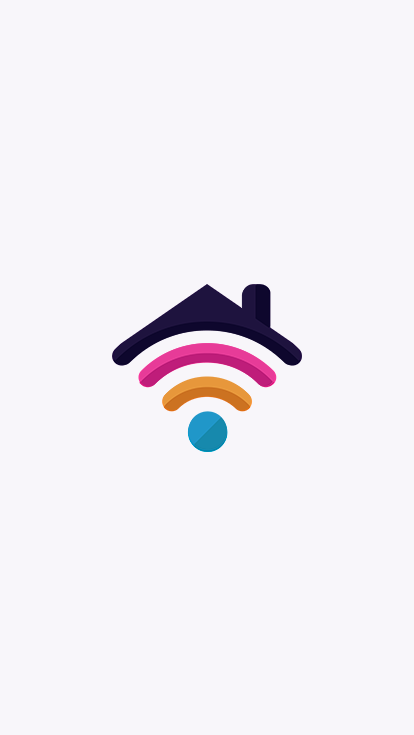
\includegraphics[scale=0.35]{1}
                    \caption{Splash Screen}
                    \label{fig:splash}
                \end{figure}

                % Menu
                \graphicspath{ {figuras/} }
                \begin{figure}[h]
                    \centering
                    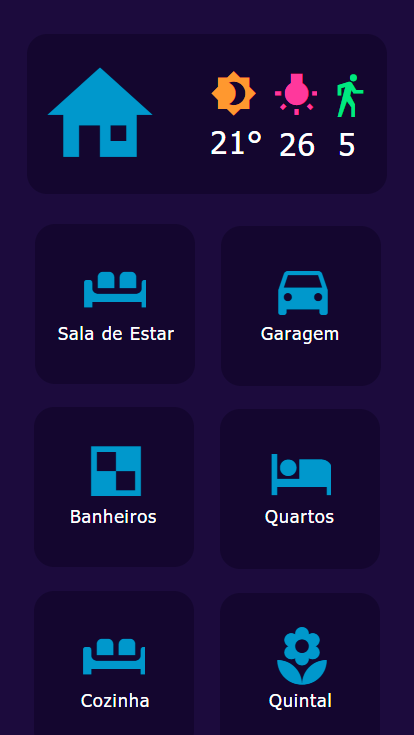
\includegraphics[scale=0.35]{2}
                    \caption{Menu Inicial}
                    \label{fig:menu}
                \end{figure}

                % Cômodo Específico
                \graphicspath{ {figuras/} }
                \begin{figure}[h]
                    \centering
                    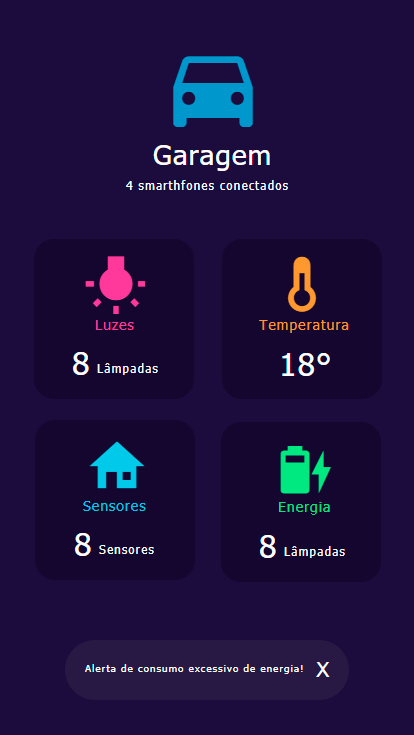
\includegraphics[scale=0.35]{3}
                    \caption{Cômodo Específico}
                    \label{fig:comodo}
                \end{figure}
